\documentclass[12pt,letterpaper,noanswers]{exam}
\usepackage[usenames,dvipsnames,svgnames,table]{xcolor}
\usepackage[margin=0.9in]{geometry}
\renewcommand{\familydefault}{\sfdefault}
\usepackage{multicol}
\pagestyle{head}
\definecolor{c03}{HTML}{FFDDDD}
\header{AM 22b Class 22}{Updated \today.}{Skill Check}
\runningheadrule
\headrule
\usepackage{graphicx} % more modern
\usepackage{amsmath} 
\usepackage{amssymb} 
\usepackage{hyperref}
\usepackage{tcolorbox}
\usepackage[numbered,autolinebreaks,useliterate]{mcode}

\newcommand{\mb}[1]{\underline{#1}}

\begin{document}
 \pdfpageheight 11in 
  \pdfpagewidth 8.5in

% Name: \rule{2.5in}{0.5pt}
% \vspace{4mm}


\begin{questions}
\question Assume $x,y>0$.  For $\mb F = y +\frac{1}{x^2}\mb j$, decide if
\begin{parts}
\item the vectors in the vector field are

\begin{oneparcheckboxes}
\choice parallel to the $x$-axis
\choice parallel to the $y$-axis
\choice neither
\end{oneparcheckboxes}

\part As $x$ increases the length of the vectors

\begin{oneparcheckboxes}
\choice increases
\choice decreases
\choice neither
\end{oneparcheckboxes}

\part As $y$ increases the length of the vectors

\begin{oneparcheckboxes}
\choice increases
\choice decreases
\choice neither
\end{oneparcheckboxes}
\end{parts}

\vspace{0.5in}

\item For $\mb v = y\mb i + x\mb j$,
\begin{parts}
\item find the system of differential equations associated with the vector field.
\vspace{0.6in}
\item Does the flow $x(t) = a(e^t+e^{-t}), y(t) = b(e^t-e^{-t})$ satisfy the system?  \emph{Show your calculation steps}
\end{parts}
\vfill

\item Do you expect the sign of the line integral for the pictured vector field and given curve to be positive, negative, or zero?

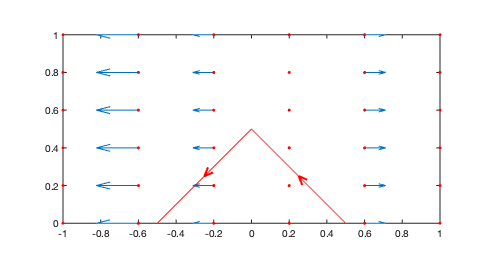
\includegraphics[width=4in]{img/C21lineintegral-p3.png}

Provide justification.

\vfill

\end{questions}

\end{document}